\documentclass[submission,copyright,a4]{eptcs}
\providecommand{\event}{WWV 2012}
\usepackage{breakurl}

\usepackage[utf8]{inputenc} % set input encoding (not needed with XeLaTeX)

\usepackage{graphicx} % support the \includegraphics command and options

%%% PACKAGES
\usepackage{booktabs} % for much better looking tables
\usepackage{array}    % for better arrays (eg matrices) in maths
\usepackage{paralist} % very flexible & customisable lists (eg. enumerate/itemize, etc.)
\usepackage{verbatim} % adds environment for commenting out blocks of text & for better verbatim
\usepackage{subfig}   % make it possible to include more than one captioned figure/table in a single float
\usepackage{listings}
\usepackage{xspace}

%%% HEADERS & FOOTERS
\usepackage{fancyhdr} % This should be set AFTER setting up the page geometry
\pagestyle{fancy} % options: empty , plain , fancy
\renewcommand{\headrulewidth}{0pt} % customise the layout...
\lhead{}\chead{}\rhead{}
\lfoot{}\cfoot{\thepage}\rfoot{}

\lstset{language=erlang,
        basicstyle=\footnotesize\ttfamily,
        columns=flexible,
        %tabsize=2,
        %numberbychapter=false,
        captionpos=b,
        %commentstyle=,
        %basewidth=0.51em,
        frame=single,
        %framesep=2pt,
        %frameround=tttt,
        breaklines=true,
        breakatwhitespace=true}

\newcommand{\LET}{\texttt{?LET}\xspace}

\title{Automatic WSDL-guided Test Case Generation\\
       for Property-Based Testing of Web Services}
\author{Leonidas Lampropoulos \and Konstantinos Sagonas}
\def\titlerunning{Automatic WSDL-guided Test Case Generation for Property-Based Testing of Web Services}
\def\authorrunning{L. Lampropoulos and K. Sagonas}

\begin{document}
\maketitle

\begin{abstract}
With web services already being key ingredients of modern web systems,
automatic and easy-to-use but at the same time powerful and expressive
testing frameworks for web services are increasingly important. Our
work aims at fully automatic property-based testing of web services:
ideally the user only specifies properties that the web service is
expected to satisfy, in the form of input-output relations, and the
system handles all the rest. In this paper we present in detail the
component which lies at the heart of this system: how the WSDL
specification of a web service is used to automatically create test
case generators that can be fed to PropEr, a QuickCheck-like
property-based testing tool, to create structurally valid random
testcases for its operations. Although the process is fully automatic,
our tool optionally allows the user to easily modify its output to
either add semantic information to the generators or write properties
that test for more involved functionality of the web services.
\end{abstract}


\section{Introduction}


% Web services + their testing

Web services are an essential part in designing a modern web system, 
especially since the appearance of the System Oriented Architecture (SOA)
model. Testing them, however, is an extremely slow process, mainly due to
the overly verbose nature of the XML SOAP messages involved. Writing 
testcases by hand is not a practical option, while existing tools for 
testing Web Services help speed up the proccess, but in our opinion fail 
to assist the tester in testing for involved web service functionality
in an easy and straightforward manner.

% Property based testing + PropEr

One approach that could be used to achieve this, is property-based testing (PBT).
The idea of expressing properties a program must satisfy in the form of 
input-output relations, and present the general structure of valid input 
messages, while letting the system handle the creation of progressively more 
complex testcases to find a counter-example for the property, is creating a 
growing fan base, especially in functional programming communities where 
tools such as QuickCheck (Haskell) or PropEr (Erlang) exist. Property-based 
testing applied to web services shares the same problem as other testing 
approaches: the generators would be most cumbersome to write manually. This is
where our tool comes in. Automatically creating generators for PropEr based on 
the WSDL specification of the web service, while also allowing for easy 
modification of them and use in writing expressive properties is our ultimate goal.

% What this paper does + generation techniques

In this paper we describe the methods used to handle fully automatic
test case generation based on the WSDL specification of a web service.
This idea has already appeared in a number of papers, however the 
related tools have yet to mature, while our design can lead to much 
deeper and more thorough testing possibilities because of the integration
with PropEr. In addition, we present some example uses of these generators 
in automatically testing web services for unexpected behaviors. 

% Paper outline

The rest of the paper is organized as follows.
The next section presents the proposed system architecture of the final 
product. In addition we briefly introduce the key components used to 
create our tool, such as PropEr, Yaws and xmerl.
Section 3 describes the techniques used to handle automatic creation of
test case generators and properties, along with some examples to show 
the form of the output code. 
In section 4, we show how to use our tool to test a single operation of 
a web service, fully automatically.
Section 5 compares our work with related research and tools already 
available, while the last section draws conclusions and presents ideas 
for future work.

%We describe an extension of PropEr to accomodate WSDL-guided property-based testing of web services. This extension receives the URL of a Web Service (or more accurately the url of the Web Service's WSDL specification), parses the specification and creates an output file containing generators and properties for all the SOAP Web Service operations. The output file can be automatically compiled and used for response testing of Web Services with random, yet structurally valid testcases. In addition, the automatically created PropEr generators and properties can be easily modified, allowing the user to write properties the Web Service should satisfy, utilizing the full power of Erlang and PropEr.

\section{System Architecture}


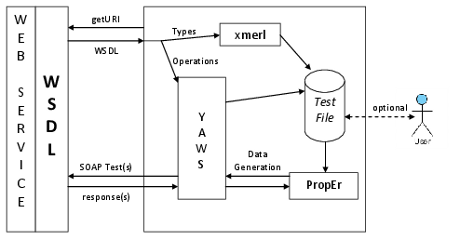
\includegraphics{PropErWebFramework.png}

The picture above shows the architecture of our testing framework. Firstly, we get the WSDL specification of the Web Service. This specification is then fed into two different erlang tools, Yaws and Xmerl, which will be briefly described later on in this section. Using xmerl, we extract all the type information associated with the WSDL specification, while using yaws we extract all supported (SOAP) operations. The extracted information is then used to create a testing file (erlang code) that contains PropEr generators and properties ready for use. Then, the user can (optionally) modify the testing file to add his own properties or refine the generators. The testing file is then given as input to PropEr, which generates random testcases, invokes the Web Service (using Yaws as a SOAP wrapper) and then analyzes the result.

%To use the extension required are an Erlang distribution (with xmerl), Proper and Yaws.
%To run some of the examples below, Eclipse and Tomcat have been used, but any means of creating a Web Service should be an option.

\subsection{WSDL}

WSDL is the leading specification for web services in XML format, describing the web service in full: operations, input and output message types, locations, bindings, port types etc. 

Every WSDL specification contains (or references) an XSD schema inside, describing the types of the messages needed to invoke the Web Service. The types of these messages are divided in two large categories: simple and complex types. Simple types can be either primitive datatypes, such as floats, ints, strings, etc., aggregates of the above, such as lists and unions, or restricted versions of them, like enumerations or range constraints. Complex types on the other hand are derived (extented or restricted) based on other types, which in turn are either simple or complex. Usually, complex types are created by forming element aggregates - sequences or choices. 

In addition to types, a WSDL specification also describes the operations the Web Service provides, along with information linking the input and output messages of an operation with types defined in the XSD Schema. 

\subsection{PropEr}

\subsection{Yaws}

Yaws is the most widely used Erlang HTTP webserver. Yaws uses an XML parser called Erlsom to handle its soap message encoding/decoding, a parser module faster and more user friendly than the xmerl module of the Erlang distribution, imposing however a few additional limitations. In our framework, Yaws is used at two different times: in the beginning, in order to extract all the supported SOAP operations from the WSDL specification, and during the actual testing phase, as an intermediary between PropEr and the Web Service, wrapping the data generated by PropEr in valid SOAP structure, invoking a Web Service operation with the formed SOAP message, retrieving the result and returning it in the form of an erlang tuple to PropEr for further analysis.

\subsection{xmerl}

Xmerl is an XML parser, included in the erlang/OTP distribution. It transforms any XML to a (rather verbose) erlang structure containing all the information contained in the original XML document. In our framework, xmerl is used to parse the XSD Schema of the WSDL specification, in order to extract the typing information nedded to create PropEr generators.

\section{Automatic Creation of Generators and Properties}

The main idea behind the extension is to use PropEr to do property based testing on web services. This extension helps the user by creating generators, sample properties and call functions so that the user focuses on the important task - writing the property. 

\subsection{Automatic Creation of Test Case Generators from WSDL Types}

The most important part of our tool is the automatic creation of PropEr generators from the types described in the WSDL specification. To that end, we introduce an intermediate Erlang representation of the WSDL types; a representation that can be directly mapped to PropEr generators, while at the same time is easier to work with and handles all constraining facets of the XSD Schema. The following XSD Schema is an example of a type specification of a Web Service which we will use to show how the generators are created.

\begin{lstlisting}
  <complexType name="ProductType">
    <sequence>
      <element maxOccurs="1" minOccurs="1" name="name" type="xsd:string"/>
      <element maxOccurs="1" minOccurs="1" name="price" type="xsd:positiveInteger"/>
      <element maxOccurs="1" minOccurs="1" name="shipInfo" type="impl:ShipInfo"/>
    </sequence>
  </complexType>
  <simpleType name="PaymentType">
    <restriction base="xsd:string">
      <enumeration value="visa"/>
      <enumeration value="paypal"/>
      <enumeration value="deposit"/>
    </restriction>
  </simpleType>
  <complexType name="ShipInfo">
    <sequence>
      <element maxOccurs="1" minOccurs="1" name="paymentInfo" type="impl:PaymentType"/>
      <element maxOccurs="1" minOccurs="1" name="address" type="xsd:string"/>
    </sequence>
  </complexType>
  <element name="Order">
    <complexType>
      <sequence>
        <element maxOccurs="unbounded" minOccurs="1" name="products" type="impl:ProductType"/>
      </sequence>
    </complexType>
  </element>
  <element name="Product" type="impl:ProductType"/>
\end{lstlisting}

% Na mpei edw kapoia perigrafi tou parapanw sximatos i den xreiazetai?

Suppose we want to create a generator for an operation \texttt{"placeOrder"} of a Web Service that takes as an argument a single element \texttt{"Order"}. In the front end of the implementation, we use the information provided by the xmerl module after parsing the schema to go through all elements and their types recursively, passing through all the nodes of the XSD schema in a DFS style. In every such node, we create a tuple that contains both name and type information for the node and all its succesors. 

Simple types yield tuples that contain only type information, along with an atom to facilitate compatibility with Erlsom and Yaws. In our example, we encounter three different simple types. Two of them, namely xsd:string and xsd:positiveInteger represent primitive datatypes of the WSDL specification, where as "tns:PaymentType" is a user defined simple type - a restriction upon the string type. The tuples associated with these types in our tool are:

\begin{lstlisting}
xsd:positiveInteger : {erlsom_string, integer, {1, inf}}
\end{lstlisting}

The positiveInteger primitive datatype is mapped by default to the above tuple. The first argument \texttt{'erlsom\_string'} states that for compatibility with Yaws it must be converted to String before wrapped in valid SOAP structure, the second argument that the base PropEr generator is \texttt{integer()} and the last denotes the range (minimum and maximum value of the generated value) is between 1 and infinity. 

\begin{lstlisting}
xsd:string : {list,{{range,0,inf},{erlsom_int,integer,{32,127}}}}
\end{lstlisting}

This simple type shows how strings are mapped to intermediate tuples. The first argument shows that the entire tuples representes a list and the second argument specifies the length of the list (in this case it is arbitrary) and the inner type (its intermediate represantation) of the list (in this case a character - since strings in erlang are lists of numbers, the generator creates such lists with integers in the range 32 - 127, printable characters in the ascii table).

\begin{lstlisting}
tns:PaymentType: {elements,["visa","paypal","deposit"]}
\end{lstlisting}

The final simple type is a user defined restriction upon the basic string datatype, defining an enumeration of the acceptable values. As a result the only acceptable values are "visa", "paypal" or "deposit" and the intermediate tuple denotes just that.

Elements yield tuples that contain type and naming information. The naming information contains the name of the element (if it exists) as well as namespace information of the XSD Schema. For example the "price" element:

\begin{lstlisting}
<element maxOccurs="1" minOccurs="1" name="price" type="xsd:positiveInteger"/>
\end{lstlisting}

is represented with the tuple:

\begin{lstlisting}
{{price,['ProductType'],'http://bar'}, {erlsom_string,integer,{1,inf}}}
\end{lstlisting}

Finally complex types usually define aggregates of simple types. In our example, we encounter three complex types, all of which combine child elements with a "sequence" combinator. For example, the "ShipInfo" complex type is represented as:

\begin{lstlisting}

{{'ShipInfo',[],'http://bar'},
  {tuple,
    [{{paymentInfo,['ShipInfo'],'http://bar'},
      {{'PaymentType',[],'http://bar'},
       {elements,["visa","paypal","deposit"]}}},
     {{address,['ShipInfo'],'http://bar'},
      {list, {{range,0,inf}, {erlsom_int,integer,{32,127}}}}}]}}
\end{lstlisting}

This shows that besides the name information, the intermediate representation consists of a "tuple" atom - indicative of the "sequence" combinator and a list of the child intermediate tuples. In this case, since the minOccurs and maxOccurs attributes for the child elements are both equal to 1, we include the child generator as is. In case these attributes implied a collection (eg unbounded), we would need to wrap the inner generators in a list intermediate tuple.

% Back end now

The mapping of the intermediate tuples to PropEr generators is pretty straightforward by construction. Special care is only needed to ensure names for all generators are unique. To that end we use the full path up to the current node as prefix, leading to rather long but descriptive and unique names. The generators produced for the previous example by our tool are:

\begin{lstlisting}
generate_Order_1_products_ProductType_name() -> 
  list(integer(32, 127)).

generate_Order_1_products_ProductType_price() ->  
  ?LET(Gen, integer(1,inf), integer_to_list(Gen)).

generate_Order_1_products_ProductType_shipInfo_ShipInfo_paymentInfo_PaymentType() -> 
  elements(["visa", "paypal", "deposit"]).

generate_Order_1_products_ProductType_shipInfo_ShipInfo_address() -> 
  list(integer(32, 127)).

generate_Order_1_products_ProductType_shipInfo_ShipInfo() -> 
  ?LET(
    {Pr_Order_1_products_ProductType_shipInfo_ShipInfo_paymentInfo_PaymentType,
     Pr_Order_1_products_ProductType_shipInfo_ShipInfo_address},
    {generate_Order_1_products_ProductType_shipInfo_ShipInfo_paymentInfo_PaymentType(),
     generate_Order_1_products_ProductType_shipInfo_ShipInfo_address()},
    [Pr_Order_1_products_ProductType_shipInfo_ShipInfo_paymentInfo_PaymentType,
     Pr_Order_1_products_ProductType_shipInfo_ShipInfo_address]
  ).

generate_Order_1_products_ProductType() -> 
  ?LET(
    {Pr_Order_1_products_ProductType_name, 
     Pr_Order_1_products_ProductType_price, 
     Pr_Order_1_products_ProductType_shipInfo_ShipInfo},
    {generate_Order_1_products_ProductType_name(), 
     generate_Order_1_products_ProductType_price(), 
     generate_Order_1_products_ProductType_shipInfo_ShipInfo()},
    [Pr_Order_1_products_ProductType_name, 
     Pr_Order_1_products_ProductType_price, 
     Pr_Order_1_products_ProductType_shipInfo_ShipInfo] 
  ).

generate_Order_1_products() -> 
  ?LET(Len, range(1, inf), vector(Len, generate_Order_1_products_ProductType())).

generate_Order_1() -> 
  ?LET(Pr_Order_1_products, generate_Order_1_products(), [Pr_Order_1_products]).
\end{lstlisting}

The above code reveals the generation method. Simple types are mapped almost directly like the "PaymentType", with special care taken if needed to add a wrapper that converts the generated data to string if that is required by Yaws. Complex types on the other hand, need to be represented as lists for Yaws to accept them, and we use \LET macros to that end. 
% Include the following or not?
PropEr would allow for simplicity to create less verbose versions of these generators with a little extra care for unique naming. For example the last generator could have been written as:

\begin{lstlisting}
generate_Order_1() ->
  [generate_Order_1_products()].
\end{lstlisting}

While in such a small example this would appear preferable, it actually makes things more difficult for the user, should he want to modify the generated test data or the generators. The importance of the \LET macro can be seen in the following example: Suppose a Web Service has an operation that takes as input an element with an "ISBN" field amongst others (a semantically valid ISBN is a unique identifier for a book and consists of 10 single digits, the last of which is determined by the previous nine via a congruence). For such a Web Service, our tool would generate code of the following form:

\begin{lstlisting}
generate_opName() ->
  ?LET(
    {Pr_opName_ISBN,
     ...},
    {generate_opName_ISBN(),
     ...},
    [Pr_opName_ISBN,
     ...]
  ).
\end{lstlisting}

Where the generate\_opName\_ISBN() generator would create a 10-member list of single digit integers. With a small function that changes the first digit so that the ISBN congruence is satisfied (eg ISBNize()), one could rewrite the generator as:

\begin{lstlisting}
generate_opName() ->
  ?LET(
    {Pr_opName_ISBN,
     ...},
    {generate_opName_ISBN(),
     ...},
    [ISBNize(Pr_opName_ISBN),
     ...]
  ).
\end{lstlisting}

This is only possible with the use of the \LET macro that allows you to modify and combine the generated data. 


\subsection{Automatic Creation of Properties from WSDL Operations}

In addition to automatically creating generators, our tool also creates a couple of functions for each Web Service operation, that invokes this operation using Yaws. Also, it creates a small property to test the Web Service always responds for random testcases, with a well formed SOAP message. This approach allows us to find most basic errors in the Web Service implementation identifying SOAP:Fault structures, since SOAP Faults are analogous to Java exceptions. 

For the XSD Schema of the previous section, our tool creates the following code:

\begin{lstlisting}
call_placeOrder(Arguments) ->
  inets:start(),
  WSDL = yaws_soap_lib:initModel(?WSDL_URL),
  yaws_soap_lib:call(WSDL, "placeOrder", Arguments).
    
call_placeOrder(WSDL, Arguments) ->
  yaws_soap_lib:call(WSDL, "placeOrder", Arguments).
\end{lstlisting}

These functions both invoke the "placeOrder" operation of the Web Service feeding "Arguments" to Yaws to wrap in a SOAP message. The difference between the two, is that the first function attempts to start the inets module (an erlang module that includes an HTTP client) and also parses the WSDL specification of the Web Service in order to create the model Yaws needs in order to make the actual call. The second function takes the WSDL model of the Web Service as an argument and invokes the operation directly, thus being more efficient than the first.

Finally, the property that is automatically created is the following:

\begin{lstlisting}
prop_placeOrder_responds() ->
  ?FORALL(Args, generate_Order_1(),
    begin
      Result = call_placeOrder(Args),
      case Result of 
        {ok, _Attribs, [#'soap:Fault'{}]} -> false;
        {ok, _Attribs, _Result_record} -> true;
        _ -> false
      end
    end).
\end{lstlisting}

The responds property is a ?FORALL macro, creating random data for the Web Service using the PropEr generators previously created, uses the above calling functions to invoke the operation and finally does a pattern matching on the resulting tuple. If Yaws encountered some problem in parsing the SOAP messages an \{error, Reason\} tuple is returnedand the property is not satisfied. Also, if a 'soap:Fault' struct is encountered as the body of the Web Service SOAP response, the Web Service failed to response correclty and the property is also not satisfied. In any other case, Yaws was able to parse a valid SOAP answer, so we assume the Web Service responded correctly and move on to the next testcase.

For the resulting file to be directly compilable, we include all headers, defines and imports needed by erlang. In addition a function called "answer\_placeOrder" is created which shows how to extract the answer (record) that is returned by Yaws. Finally, the extension also uses erlsom to output a small .hrl (erlang library) file that describes the records used for the responses of the Service. We will see how these can be used in later sections.

\section{Response Testing of Web Services}

The first kind of testing, that works without any user additions is response testing. Basically, the output file created by the extension contains a property that invokes an operation of the web service with random inputs and expects an answer for each different input. This can basically check if a web service crashes for a specific input or similar unwanted behaviors. 

Let's see how to use the tool to test an existing Web Service that converts between cooking units. This free Web Service is hosted at "http://www.webservicex.net/ConvertCooking.asmx" and its WSDL specification lies in the url "http://www.webservicex.net/ConvertCooking.asmx?WSDL". 

The XSD Schema of the Web Service is the following:

\begin{lstlisting}
<s:element name="ChangeCookingUnit">
        <s:complexType>
          <s:sequence>
            <s:element minOccurs="1" maxOccurs="1" name="CookingValue" type="s:double" />
            <s:element minOccurs="1" maxOccurs="1" name="fromCookingUnit" type="tns:Cookings" />
            <s:element minOccurs="1" maxOccurs="1" name="toCookingUnit" type="tns:Cookings" />
          </s:sequence>
        </s:complexType>
      </s:element>
      <s:simpleType name="Cookings">
        <s:restriction base="s:string">
          <s:enumeration value="drop" />
          <s:enumeration value="dash" />
          ...
          <s:enumeration value="TenCan" />
        </s:restriction>
      </s:simpleType>
      <s:element name="ChangeCookingUnitResponse">
        <s:complexType>
          <s:sequence>
            <s:element minOccurs="1" maxOccurs="1" name="ChangeCookingUnitResult" type="s:double" />
          </s:sequence>
        </s:complexType>
      </s:element>
      <s:element name="double" type="s:double" />
\end{lstlisting}

Where the Cookings simple type is a large enumeration with most of the values omitted in the Schema above. Our tool creates the output file (by default "proper\_output.erl", which can be used directly to check the WS:

% Change names of functions (wsdl_handler:generate for instance)?
\begin{lstlisting}
Erlang R15B (erts-5.9) [source] [64-bit] [smp:4:4] [async-threads:0] [hipe] [kernel-poll:false]

Eshell V5.9  (abort with ^G)
1> wsdl_handler:generate("http://www.webservicex.net/
ConvertCooking.asmx?WSDL").
ok
2> c(proper_output).
{ok,proper_output}
3> proper:quickcheck(proper_output:prop_ChangeCookingUnit_responds()).
....(100 dots) .....
OK: Passed 100 test(s).
true
\end{lstlisting}

As we can see, the Cooking web service was invoked 100 times with random arguments and returned a correctly formed result each time.

Now for an example of a service that crashes, we created our own web service using eclipse and tomcat. This example will also be used later on and is based on the first PropEr publication by Manos Papadakis, about a faulty delete function.

We have a simple Java implementation of the web service:

\begin{lstlisting}
public Class Delete {
    private String delete(String in, char c, StringBuffer acc){
        if (in.equals("")) {
            return acc.toString();
        }
        else if (in.charAt(0) == c) {
            return acc.toString().concat(in.substring(1));
        }
        else {
            return delete(in.substring(1), c, acc.append(in.charAt(0)));
        }
    }
    
    public String delete(String in, String c){
        return delete(in, c.charAt(0), new StringBuffer(""));
    } 
}
\end{lstlisting}

We used this code to implement and publish a simple Web Service in tomcat. After using the PropEr extension to handle the WSDL specification of this web service, the output file was the following:

\begin{lstlisting}
-module(proper_output).

-include_lib("proper/include/proper.hrl").
-include("proper_output.hrl").

-define(PREFIX, "properns").
-define(WSDL_URL, "http://localhost:8080/DeleteProject/services/Delete?WSDL").

-export([call_delete/1, call_delete/2]).
-export([answer_delete/1]).

generate_delete_1_in() -> 
  list(integer(32, 127)).

generate_delete_1_c() -> 
  list(integer(32, 127)).

generate_delete_1() -> 
  ?LET({Pr_delete_1_in, Pr_delete_1_c},
       {generate_delete_1_in(), generate_delete_1_c()},
       [Pr_delete_1_in, Pr_delete_1_c]).

call_delete(Arguments) ->
  inets:start(),
  Wsdl = yaws_soap_lib:initModel(?WSDL_URL),
  yaws_soap_lib:call(Wsdl, "delete", Arguments).
    
call_delete(WSDL, Arguments) ->
  yaws_soap_lib:call(WSDL, "delete", Arguments).

prop_delete_responds() ->
  ?FORALL(Args, generate_delete_1(),
    begin
      Result = call_delete(Args),
      case Result of 
        {ok, _Attribs, [#soap:Fault()]} -> false; 
        {ok, _Attribs, _Result_record} -> true;
        _ -> false
      end
    end).

answer_delete({ok, _, [Answer_record]}) -> Answer_record.

% ---------- End of Auto Generated Code ---------- 
\end{lstlisting}

Calling quickcheck with this property reveals a flaw in our implementation.
\begin{lstlisting}
> proper:quickcheck(proper_output:prop_delete_responds()). 
.!
Failed: After 2 test(s).
[[46],[]]

Shrinking .(1 time(s))
[[],[]]
false
\end{lstlisting}

In our implementation we assume that the string c which is supposed to contain at its first character the character that should be removed from the string, is not empty. We have two choices to fix it, either fix our implementation, or remove this testcase from the generator. To show how easy it is to change the generators created by the extension we choose the latter: we change the generator of c to:

\begin{lstlisting}
generate_delete_1_c() ->
  ?LET(Len, range(1,1), vector(Len, integer(32,127))).
\end{lstlisting}
We could change it to range(1,inf) or actually remove the \LET macro, but we'd have to be carefull not to actually change the output of the generator to a char instead of a non-empty char list.

Now only valid testcases are created. Testing the response property again we get:
\begin{lstlisting}
> proper:quickcheck(proper_output:prop_delete_responds()).
....(100 dots) .....
OK: Passed 100 test(s).
true
\end{lstlisting}

\section{Property-based Testing of RESTful Web Services}

Restful Web Services are Web Services compliant to a few constraints, the main one having to do with state: Each request from any client must contain all the information needed by the service to handle the request. This makes property-based testing of these services relatively easy, since each test is self-contained and does not affect the outcome of other tests. 

Let's see the delete example in more depth now. 

The answer\_result function shows how to extract the Answer record from the call response. This response is in the form of an erlsom-created record, described in the .hrl file created by the wsdl\_handler. In the .hrl file we see a record: 
\begin{lstlisting}
-record('p:deleteResponse', {anyAttribs, 'deleteReturn'}).
\end{lstlisting}

This record is the record that contains the result (when there is no error).In the automatically generated code we can locate this function:

\begin{lstlisting}
answer_delete({ok, _, [Answer_record]}) -> Answer_record.
\end{lstlisting}

We see that the 'delete response' is a record containing a 'deleteReturn' value. This 'deleteReturn' value is the boolean we seek; therefore we change the answer function to:

\begin{lstlisting}
answer_delete({ok, _, [Answer_record]}) ->
  Answer_record#'p:deleteResponse'.'deleteReturn'.
\end{lstlisting}

Finally we write our property in a similar form to the respond property:

\begin{lstlisting}
prop_delete_removes_every_x() ->
  ?FORALL([_In, [C]]=Args, generate_delete_1(),
    begin
      R1 = call_delete(Args),
      Result = answer_delete(R1),
      not lists:member(C, Result)
  end).
\end{lstlisting}

% I allagi gia handling tou unbounded list (san ta string) se list(integer(32,127)) eftiakse to shrinking. Prepei na kanw kati kai gia to non empty me ena optional ?SUCHTHAT pithanotata. 

Now checking this property with proper yields the following results:

\begin{lstlisting}
> proper:quickcheck(proper_output:prop_delete_removes_every_x()).
............!
Failed: After 12 test(s).
[[33,42,111,43,99,45,67,52,122,52,38,122],[52]]

Shrinking .........(9 time(s))
[[32,32],[32]]
false
\end{lstlisting}

We see that we find a faulty testcase in just a few tests and PropEr manages to shrink it to find the essence of the bug.

Now we show another example of testing a RestFul Web Service, to show some limitations of our implementation. Going back to the Cooking service, a simple property that should be valid in it would be if we convert something and then convert the answer back we should get the initial number.

Let's change the answer function and write this property on the output file of the extension:

\begin{lstlisting}
answer_ChangeCookingUnit({ok, _, [Answer_record]}) -> 
  Answer_record#'p:ChangeCookingUnitResponse'.'ChangeCookingUnitResult'.

prop_back_and_forth_is_equal() ->
  ?FORALL([Value, From, To] = Args, generate_ChangeCookingUnit_1(),
    begin
      Result = call_ChangeCookingUnit(Args),
      Conv_val = answer_ChangeCookingUnit(Result),
      Result2 = call_ChangeCookingUnit([Conv_val, To, From]),
      Initial = answer_ChangeCookingUnit(Result2),
      Value == Initial
    end).
\end{lstlisting}

Basically, we break down the arguments to the sub-elements, invoke the Web Service, reinvoke the Web Service with the answer and the other two arguments flipped and compare the result. 

Testing this property we receive a (not unexpected) failure:

\begin{lstlisting}
> proper:quickcheck(proper_output:prop_back_and_forth_is_equal(), 5).
!
Failed: After 1 test(s).
[[45,49,46,54,50,55,56,54,56,51,51,53,48,55,51,56,50,48,55,50,54,57,52,101,45,48,49],
 [103,97,108,108,111,110,85,75],
 [116,97,98,108,101,115,112,111,111,110,85,83]]

Shrinking ...(3 time(s))
[[48,46,48,48,48,48,48,48,48,48,48,48,48,48,48,48,48,48,48,48,48,48,101,43,48,48],
 [100,114,111,112],[100,114,111,112]]
false
\end{lstlisting}

The shrinked counter-example, if viewed as a string is:

\begin{lstlisting}
["0.00000000000000000000e+00", "drop", "drop"]
\end{lstlisting}

Basically, it fails to produce the same result even if there is no change! A closer look with a few io:formats will reveal the problem : Floating point arithmetic. The floating point numbers created as arguments by proper are converted to Strings with some error in accuracy and the 2 subsequent calls include even more arithmetical errors. If we change the equality check to a small difference check (keeping in mind that erlsom represented those numbers as strings) we change the property to:

\begin{lstlisting}
prop_back_and_forth_is_equal() ->
  ?FORALL([Value, From, To] = Args, generate_ChangeCookingUnit_1(),
    begin
      Result = call_ChangeCookingUnit(Args),
      Conv_val = answer_ChangeCookingUnit(Result),
      Result2 = call_ChangeCookingUnit([Conv_val, To, From]),
      Initial = answer_ChangeCookingUnit(Result2),
      F1 = list_to_float(Value),
      F2 = list_to_float(Initial),
      abs(F1 - F2) < 0.000001
    end).
\end{lstlisting}

And checking the property now:

\begin{lstlisting}
8> c(proper_output).                                                  
{ok,proper_output}
9> proper:quickcheck(proper_output:prop_back_and_forth_is_equal()).
......( 100 dots) .....
OK: Passed 100 test(s).
true
\end{lstlisting}

\section{Related Work}
Move this after Introduction??

Here we will refer to tools like monadWS~\cite{monadWS@AST-11} and
many other such great works...

\section{Concluding Remarks}

\bibliographystyle{eptcs}
\bibliography{ws}

\end{document}
